% !TEX root = ../../I4PRJ, Grp3 - Dokumentation.tex
\section{iOS}
Dette afsnit beskriver udvalgte elementer af implementeringen, af den grafiske brugergrænseflade til iOS styresystemet. iOS-projektet kan findes i Smartpool.Application.iOS.

Implementeringen af iOS-applikationen består delvist i den visuelle implementering af brugergrænsefladen, og den kode-mæssige implementering af de bagomliggende view-klasser. Som vist i designafsnittet, implementeres view-klasserne som controller-broer, der implementerer view-interfaces angivet i præsentationslaget.

Implementeringen af view-klasserne foretages i udviklingsværktøjet Xamarin, i sproget C\#. Den visuelle implementering foretages med storyboards i Interface Builder, som er en del af Xcode-udviklingsværktøjet.

\subsection{Implementering i Interface Builder}
Storyboards er en visuel måde at designe brugergrænseflader til iOS, som kan sammenkobles med controller-klasser som "code-behind" filer. I udviklingen af iOS-applikationen blev view's i storyboardet implementeret, sammen med bro-dannende controller-klasser, som implementerer view-interfaces fra præsentationslaget.

\subsubsection{Storyboard}
På figur~\ref{fig:iosstoryboard} ses det overordnede storyboard layout. I layoutet repræsenterer kasserne UIViewController-subklasser, hvori det view de er tilknyttet vises. Layoutet definerer også de statiske overgange (vist med pile) mellem forskellige view's. Desuden indlejres en række view's i en UITabBarController, således at en Tab Bar implementering, modsat Windows brugergrænsefladen, ikke er nødvendig i iOS-implementeringen.

\begin{figure}
	\centering
	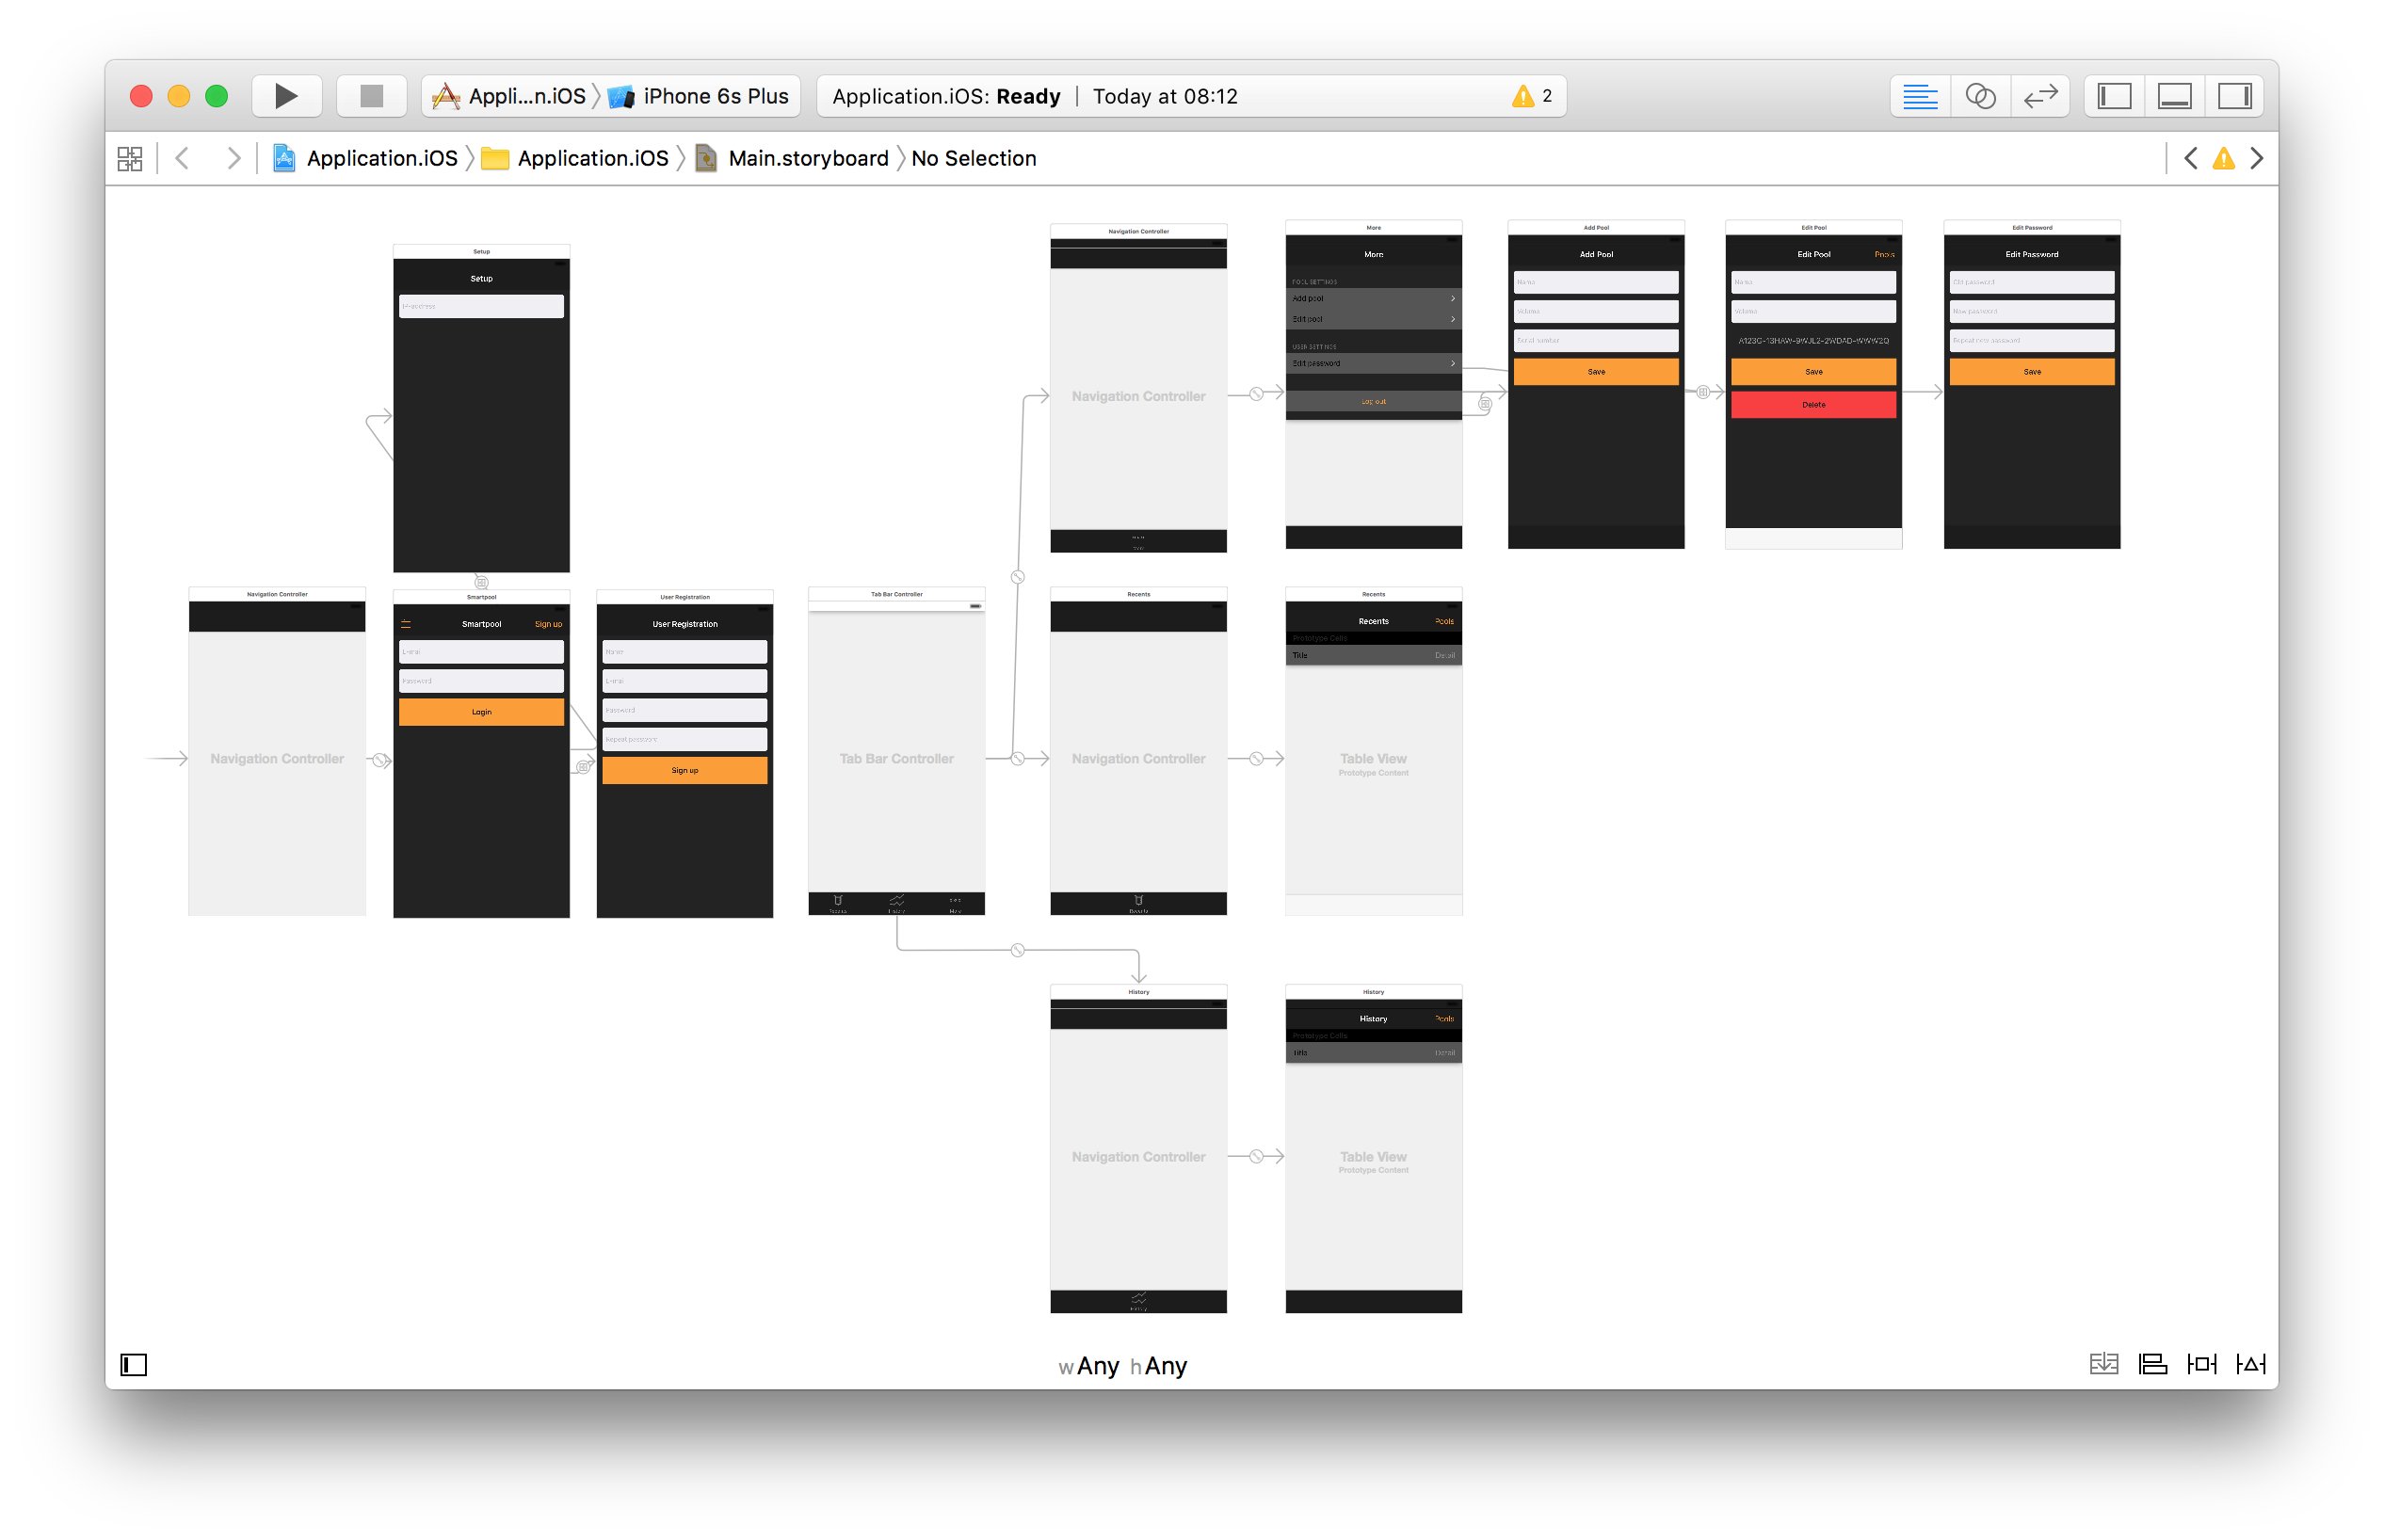
\includegraphics[width=1.0\linewidth]{figs/implementering/ios_imp_storyboard}
	\caption{Main.storyboard}
	\label{fig:iosstoryboard}
\end{figure}

\subsubsection{Layout constraints}
Layout constraints i Interface Builder muliggør skalering af brugergrænsefladen til forskellige skærmstørrelser. Hvert element i de visuelle view's er implementeret med UILayoutConstraints. På figur~\ref{fig:ios_imp_constraints} ses EditPoolViewBridge-klassens constraint-implementering (listen til venstre i billedet).

\begin{figure}
	\centering
	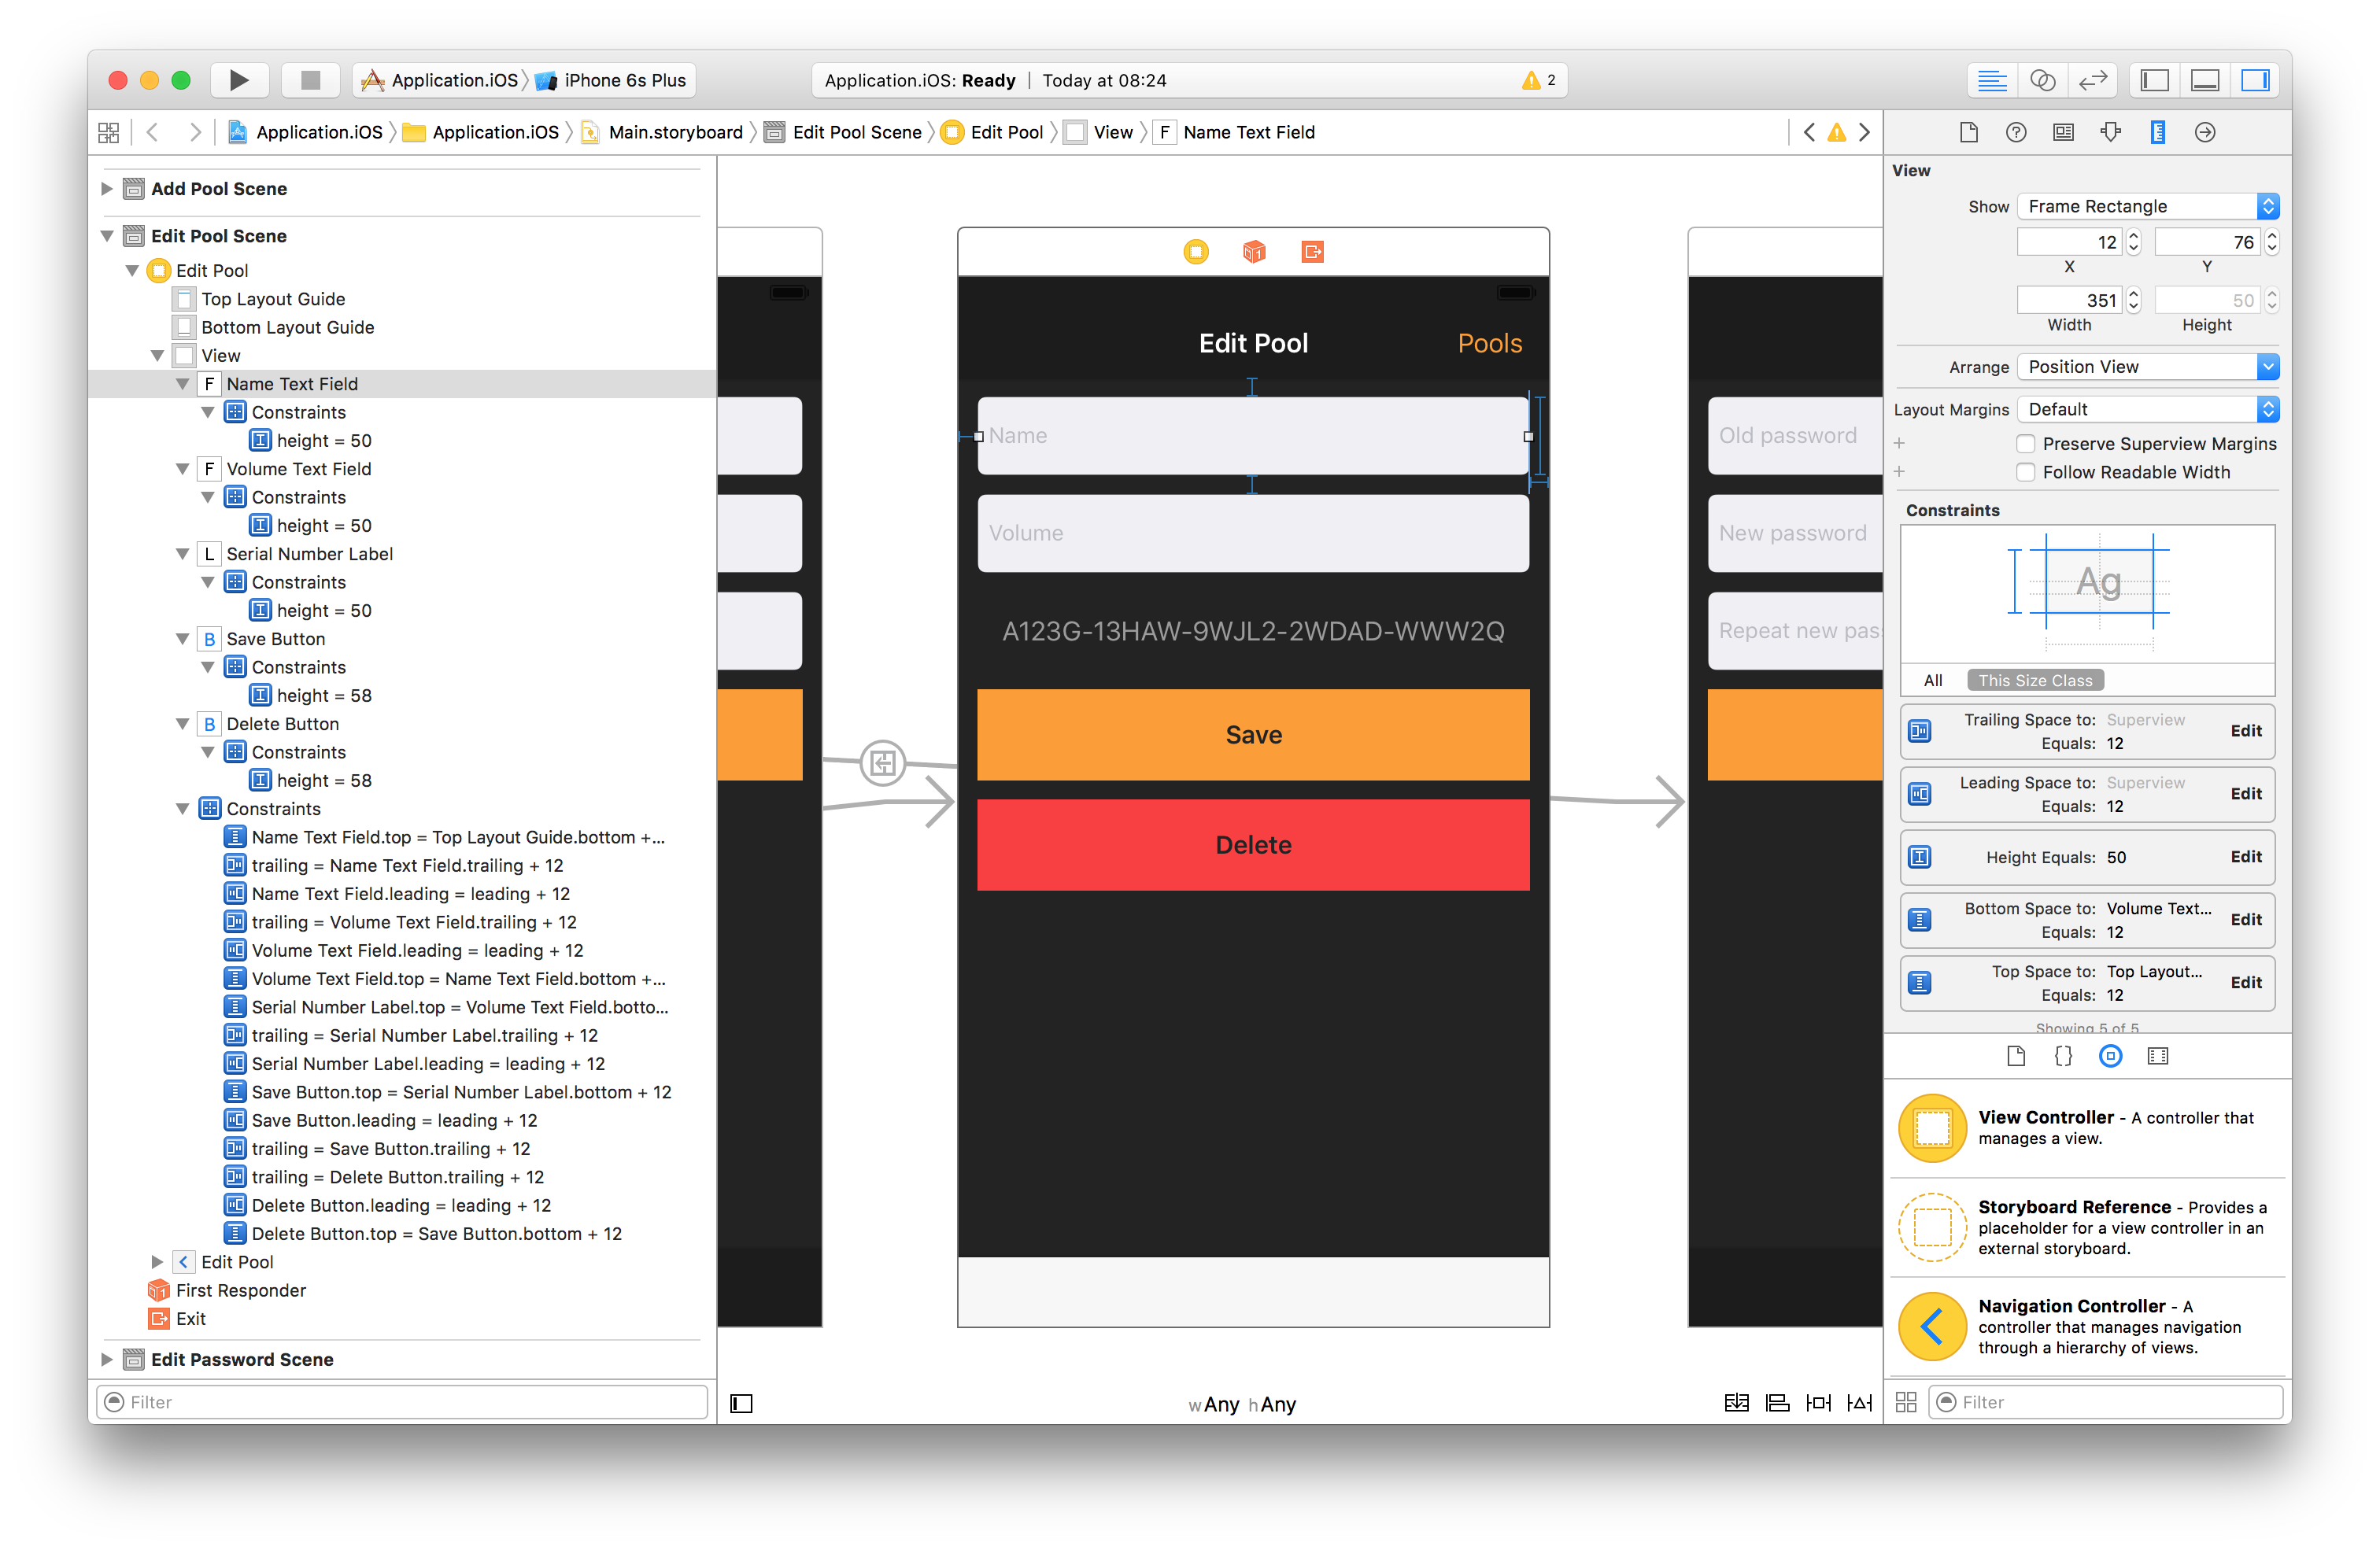
\includegraphics[width=1.0\linewidth]{figs/implementering/ios_imp_constraints}
	\caption{EditPoolViewBridge constraints}
	\label{fig:ios_imp_constraints}
\end{figure}

Til højre på figuren ses den markerede tekstboks' constraint-implementering. Her ses det, at der er implementeret constraints for elementets højde, og afstand til andre elementer.

\subsubsection{Outlets og actions}
Links mellem Interface Builder og den bagvedliggende kode, implementeres fra Interface Builder i form af IBOutlets og IBActions. IBOutlets er referencer til user interface elementerne, hvorimod IBActions er target-actions links til metode kald, eller events, i koden.

På figur~\ref{fig:ios_imp_actionsoutlets} ses outlet/action opsætningen for EditPoolViewBridge I Interface Builder. Listen af IBOutlets og Actions kan ses til højre i billedet.

\begin{figure}
	\centering
	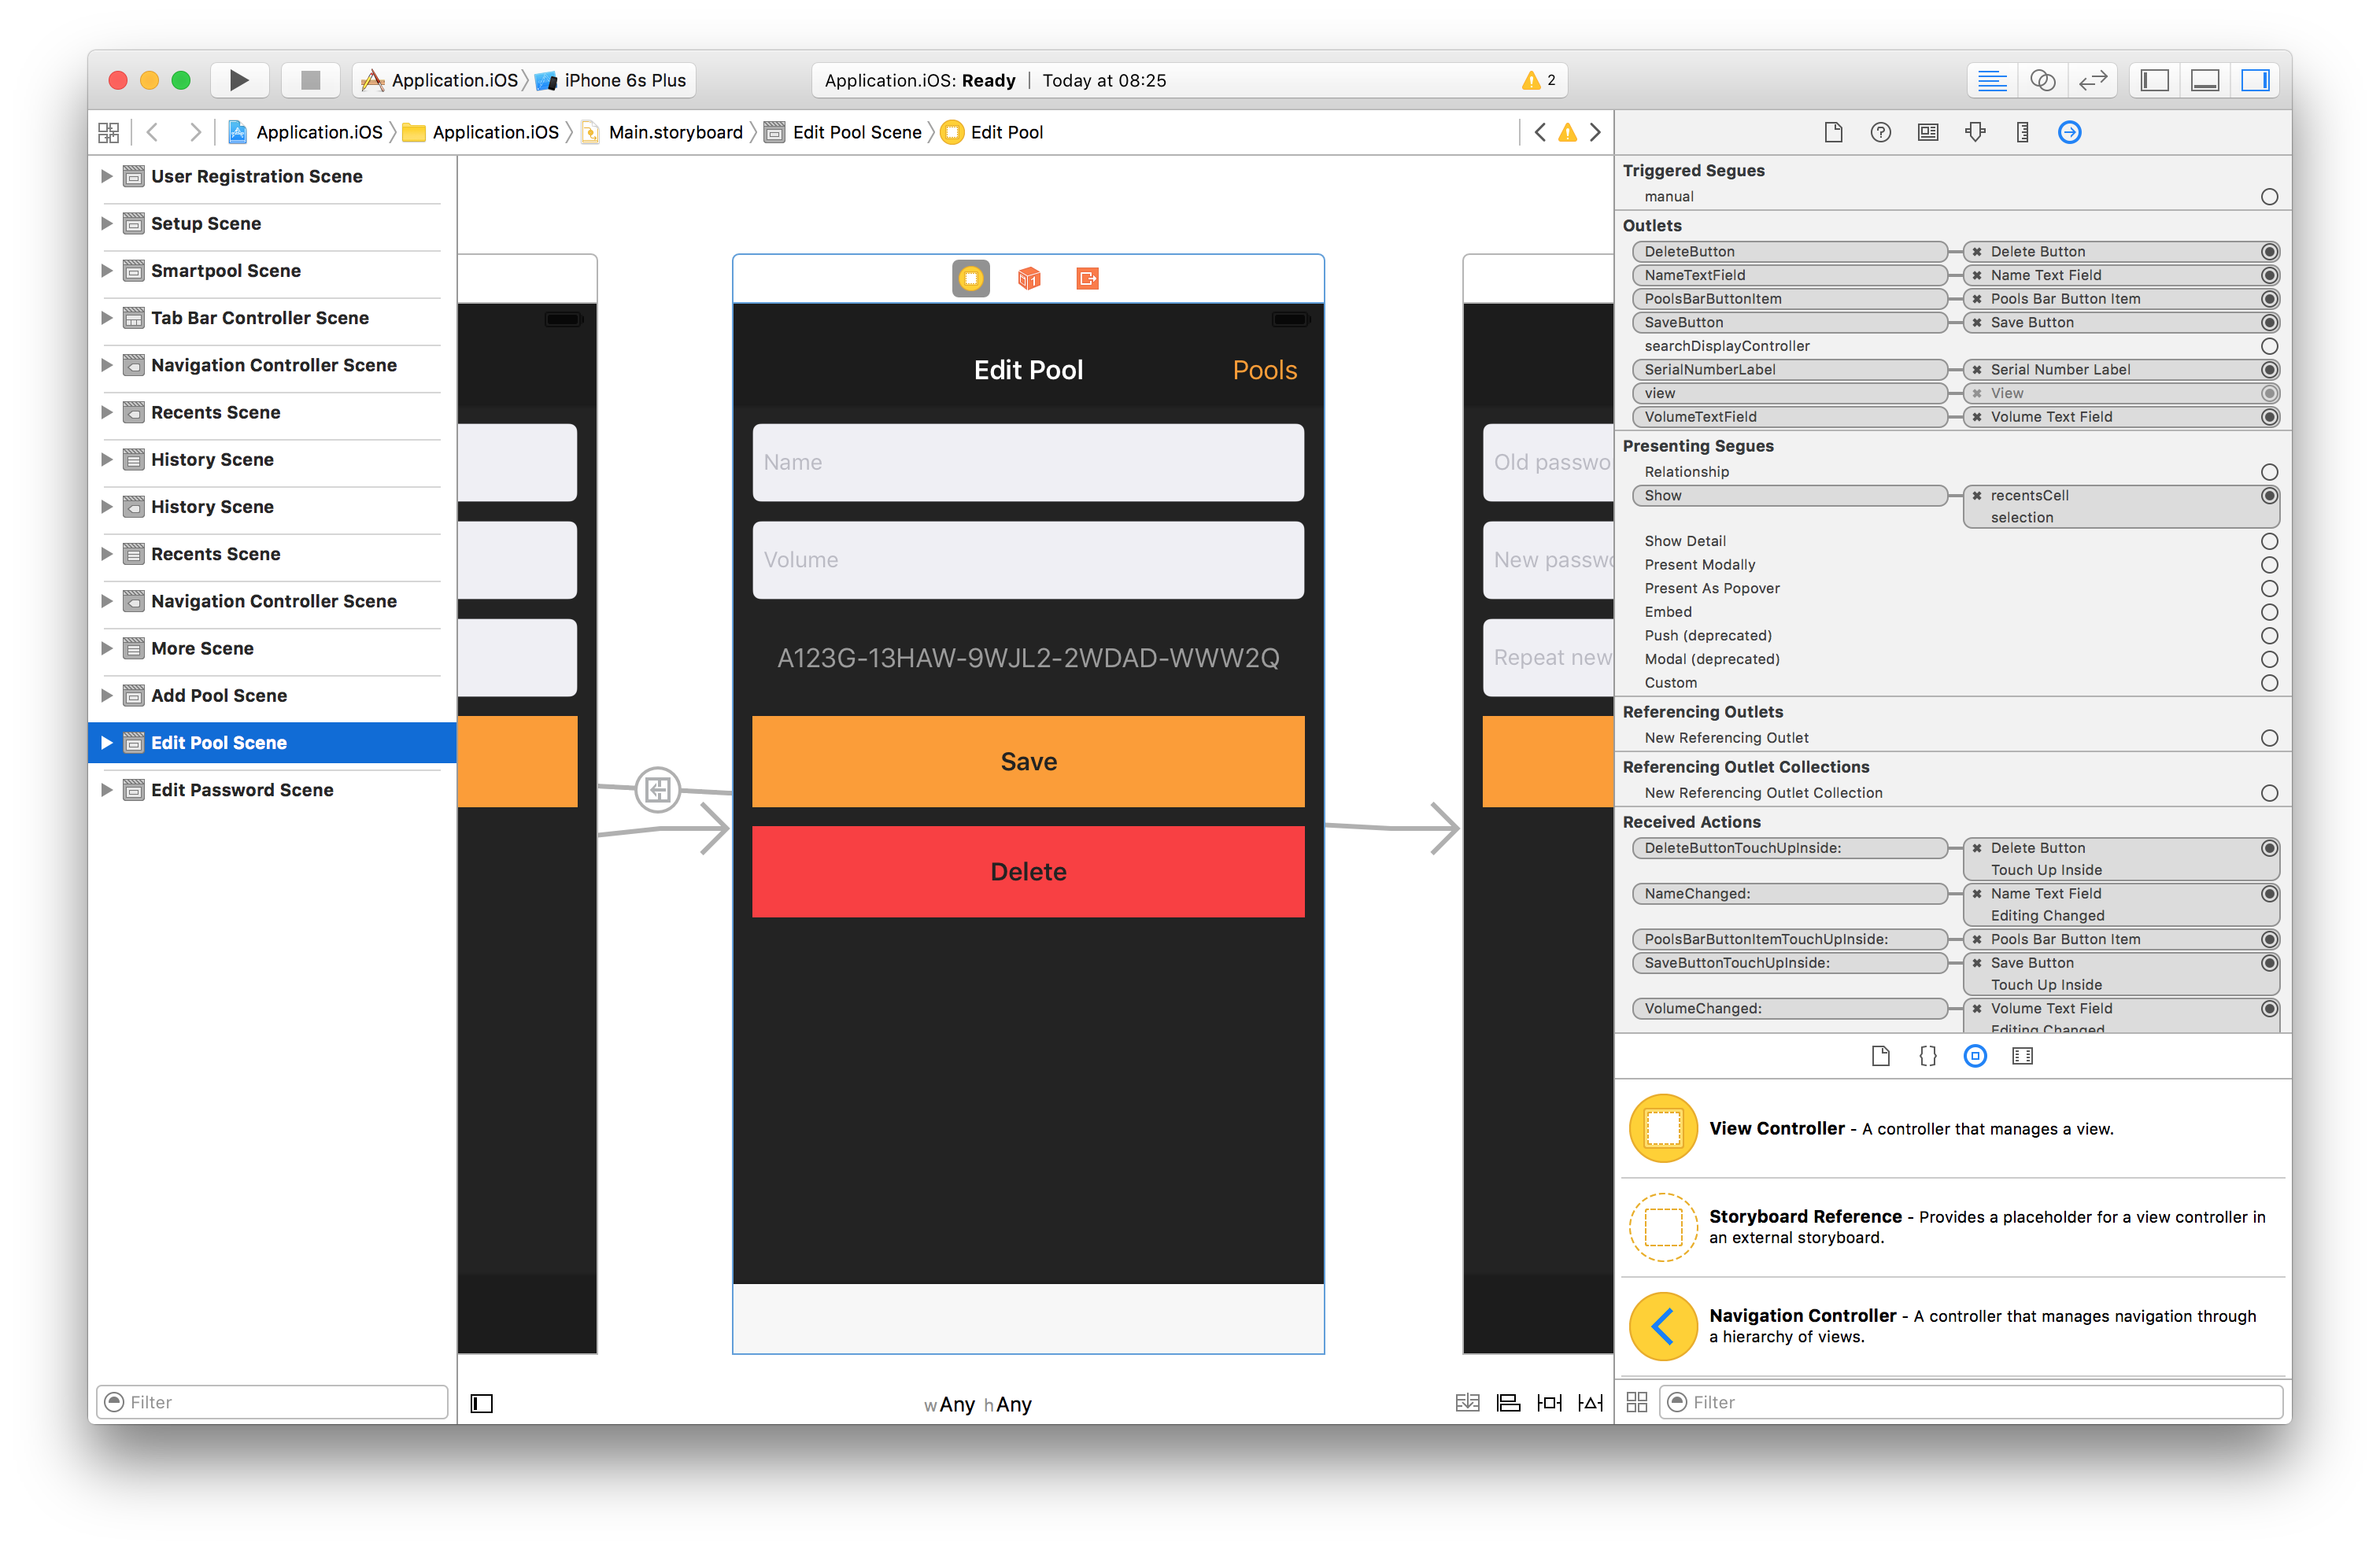
\includegraphics[width=1.0\linewidth]{figs/implementering/ios_imp_actionsoutlets}
	\caption{EditPoolViewBridge outlets og actions}
	\label{fig:ios_imp_actionsoutlets}
\end{figure}

\subsubsection{Tabel-celler}
Til StatViewController og HistoryViewController implementeres specielle tabelceller (subklasser af UITableViewCell), som kan bruges til visning af måledata. Cellerne er implementeret i en .xib-fil, med en bagvedliggende C\#-fil, på samme måde som storyboardet. På figur~\ref{fig:ios_imp_historycell} ses den visuelle implementering af HistoryViewCell.

\begin{figure}
	\centering
	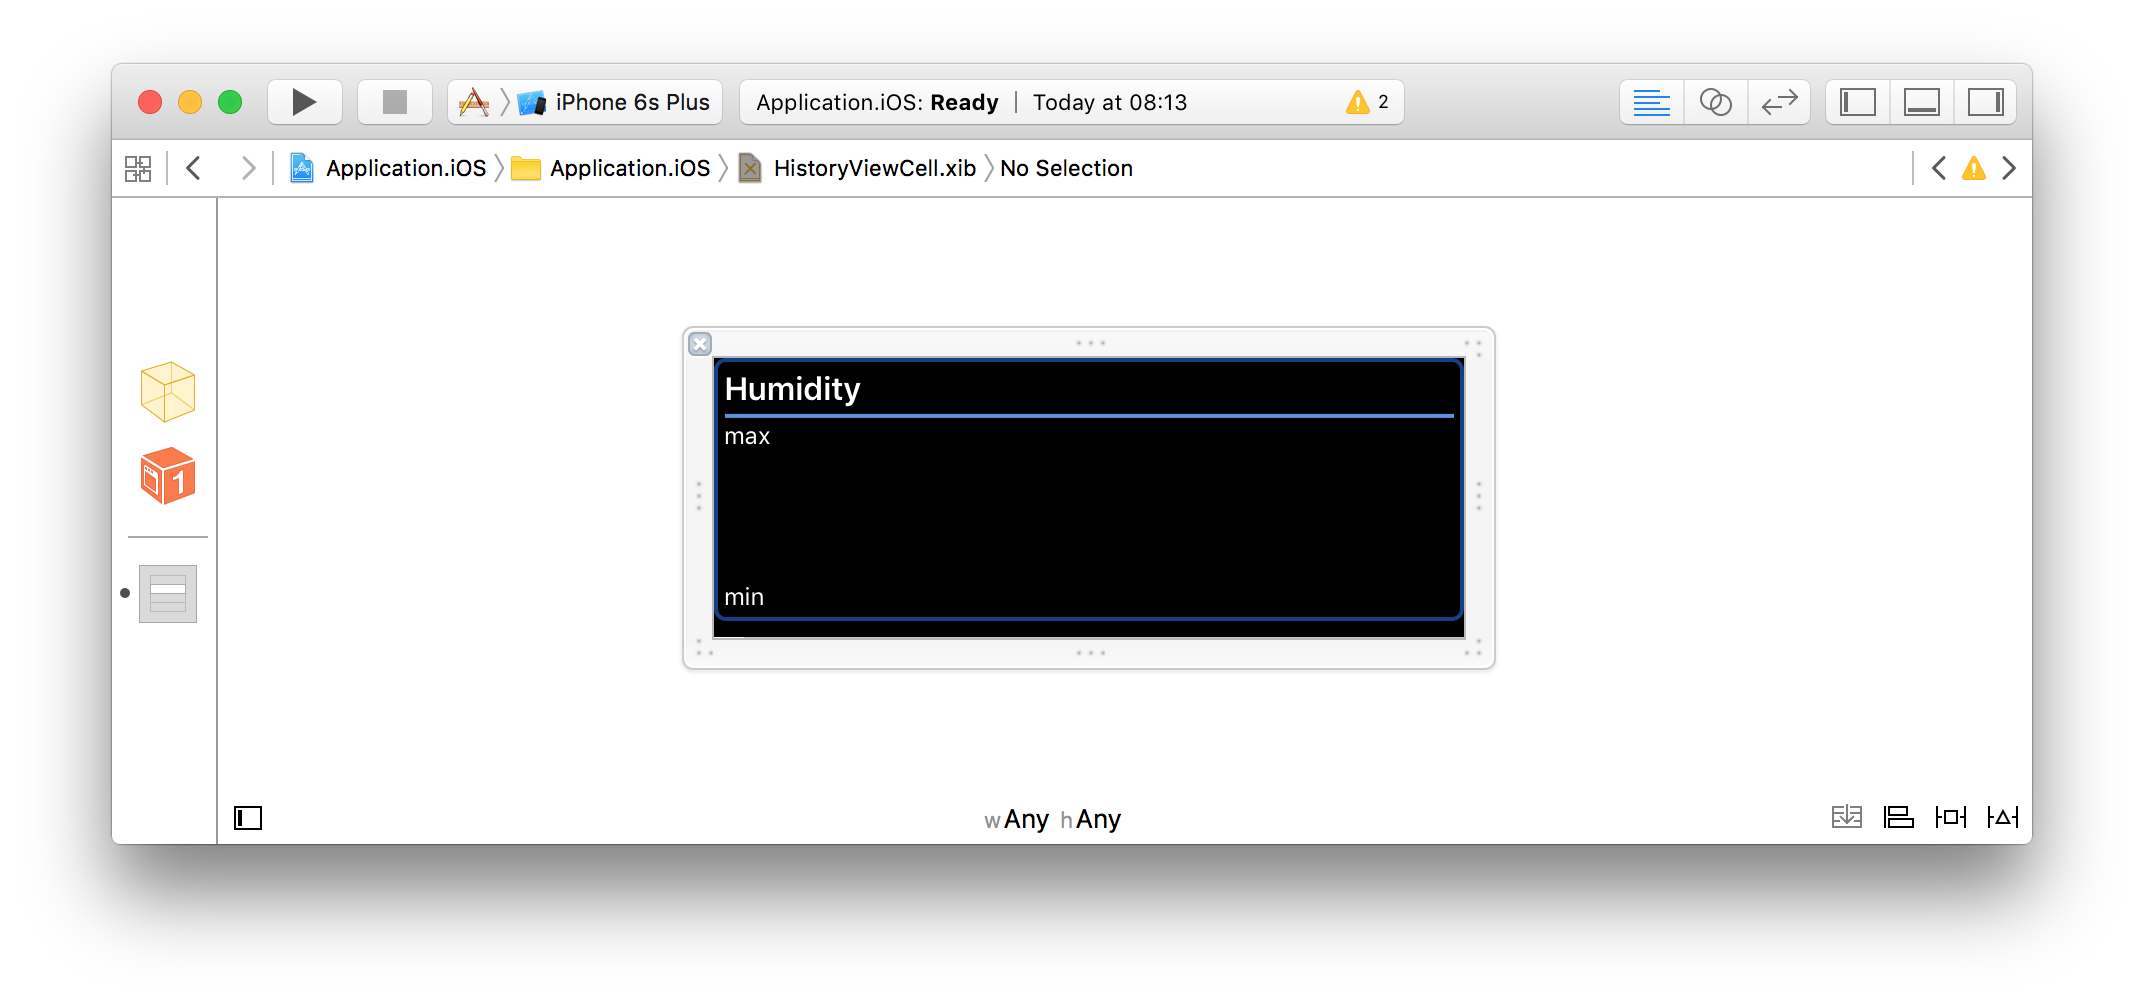
\includegraphics[width=0.8\linewidth]{figs/implementering/ios_imp_historycell}
	\caption{HistoryViewCell.xib}
	\label{fig:ios_imp_historycell}
\end{figure}

\subsection{Implementering af view-klasser}
I dette afsnit beskrives implementeringen af de brodannende controller-klasser i iOS-applikationen, som implementerer view-interfacet fra præsentationslaget.

\subsubsection{Constructor-metoder og ViewDidLoad}
Implementeringen af de forskeligge klassers constructor-metoder er meget sammenlignelig. Derfor eksemplificeres SignUpViewBridge-klassens constructor, i dette afsnit, og constructor-metoderne kommenteres herefter ikke yderligere. På listing~\ref{code:ios_impl_constructor} ses constructor-metoden.

\begin{lstlisting}[caption={SignUpViewBridge(...)},label={code:ios_impl_constructor}]
public SignUpViewBridge (IntPtr handle) : base (handle)
{
	// Initialize view controller.
	Controller = new SignUpViewController(this, iOSClientFactory.DefaultClient());
}
\end{lstlisting}

Constructor-metoden tager imod en pointer, som er en reference til klassens visuelle modpart i Main.storyboard filen, beskrevet i afsnittet om Interface Builder implementeringen. Denne constructor-metode bruges derfor, når view'et initialiseres fra et storyboard eller en .xib-fil. I metoden oprettes en instans af den presenter-klasse fra præsentationslaget, som passer til view'et. I initialiseringen af presenter-klassen, medsendes en reference til view'et, og en instans af iOS socket-klienten, som beskrives i et senere afsnit.

Da alle brodannende controller-klasser i iOS-applikationen er sub-klasser af UIViewController, UIKit's basis view controller klasse, nedarver de en ViewDidLoad metode som kaldes når view'et er indlæst i hukommelsen. I denne metode kaldes presenter-klassens ViewDidLoad-metode, for at give presenteren besked, om at view'et er initialiseret.

\begin{lstlisting}[caption={ViewDidLoad() i SignUpViewBridge},label={code:ios_impl_viewdidload}]
public override void ViewDidLoad ()
{
	base.ViewDidLoad ();
	
	// Let the controller know that the view has finished loading.
	Controller.ViewDidLoad();
}
\end{lstlisting}

\subsubsection{IBOutlets og IBActions}
Alle de implementerede view-klasser indeholder partielle implementeringer, givet ved de IBOutlets og IBActions der blev defineret i Interface Builder (se listing~\ref{fig:ios_imp_actionsoutlets}, side~\pageref{fig:ios_imp_actionsoutlets}). Under udarbejdelsen af klassernes kodeimplementering, færdigimplementeres IBOutlets og IBActions. I eksemplet givet ved listing~\ref{code:ios_impl_kodeaction}, ses hvorledes kodeimplementeringen af en IBAction ser ud.

\begin{lstlisting}[caption={Kodeimplementering af en IBAction},label={code:ios_impl_kodeaction}]
partial void emailEditingChanged (UIKit.UITextField sender)
{
	_specializedController.DidChangeEmailText(sender.Text);
}
\end{lstlisting}

Metoden kaldes når det tilhørende user interface element modtager det event, som IBAction'en blev sat op til i Interface Builder. Sender-argumentet der medsendes metoden, indeholder oplysninger om user interface elementets tilstand. I eksemplet givet ved listing~\ref{code:ios_impl_kodeaction} ses det, at senderens Text-parameter bruges til at opdatere presenter-klassen med et interface-kald.

IBOutlets bruges i kodeimplementeringen, når presenter-klassen ønsker at opdatere view'ets tilstand. I eksemplet givet ved listing~\ref{code:ios_impl_kodeaction}, ses hvorledes en IBOutlet bruges i view-klasserne. I eksemplet er variablen emailTextField en IBOutlet, der linker til et tekstfelt i user interfacet.

\begin{lstlisting}[caption={Brug af en IBOutlet i koden},label={code:ios_impl_kodeoutlet}]
public void SetEmailText(string text)
{
	emailTextField.Text = text;
}
\end{lstlisting}

Da alle view-klasserne indeholder en række af disse IBOutlet og IBAction implementeringer, som alle har formen vist i listing~\ref{code:ios_impl_kodeaction}~og~\ref{code:ios_impl_kodeoutlet}, kommenteres de ikke yderligere.

\subsubsection{Statiske views}
SignUpViewBridge, LoginViewBridge, EditPoolViewBridge, EditUserViewBridge og AddPoolViewBridge er alle statiske, i den forstand, at opsætningen af deres layout, ikke ændre sig i runtime. Det resulterer i, at der kræves meget lidt, af disse klassers implementering. De statiske views nedarver alle fra UIViewController, og implementerer det view-interface der passer til dem (SignUpViewBridge implementerer eksempelvis ISignUpView-interfacet). Implementeringen af disse klasser består hovedsageligt i, at bygge bro mellem view'et og presenter klassen, ved at implementere IBOutlet- og IBAction-kode, som vist i forrige afsnit. 

\subsubsection{StatViewBridge.cs}
StatViewBridge implementerer IStatView-interfacet. StatViewBridge nedarver, i modsætning til de statiske views, fra UIViewController sub-klassen UITableViewController. Denne UIKit controller-klasse kan bruges til at vise lister der ændre sig i runtime, som er nyttigt for StatViewBridge-klassen, da den skal kunne opdateres med måledata. I listing~\ref{code:ios_impl_statdisplay} ses implementeringen af interface-metoden DisplaySensorData. I denne metode gemmes den modtagne sensor data, så den kan bruges som data source til UITableViewController-listen.

\begin{lstlisting}[caption={DisplaySensorData(...)},label={code:ios_impl_statdisplay}]
public void DisplaySensorData(List<Tuple<SensorTypes, double>> sensorData)
{
	_sensorData = sensorData;
	_sensorData.Sort ();
	TableView.ReloadData ();
}
\end{lstlisting}

Klassen overrider en række af UITableViewController-klassens metoder, der indlæser data i view'et. De overrides der bestemmer indholdet af listens elementer, fremgår af listing~\ref{code:ios_impl_stattableor}. I GetCell-metoden opsættes en StatViewCell (StatViewCell.xib), til at vise den data der er modtaget fra presenter-klassen.

\begin{lstlisting}[caption={Overrides af UITableViewController-metoder i StatViewBridge},label={code:ios_impl_stattableor}]
public override nint RowsInSection (UITableView tableView, nint section)
{
	return _sensorData.Count;
}

public override UITableViewCell GetCell (UITableView tableView, Foundation.NSIndexPath indexPath)
{	
	var cell = tableView.DequeueReusableCell (_reuseIdentifier) as StatViewCell;
	var type = string.Format ($"{_sensorData [indexPath.Row].Item1}");
	ell.DataLabel.Text = string.Format ($"{_sensorData [indexPath.Row].Item2}") + GuiCharacter.SignForType(_sensorData [indexPath.Row].Item1);
	cell.NameLabel.Text = type;
	cell.BorderImage.Image = UIImage.FromFile (type.ToLower () + ".png");
	return cell;
}
\end{lstlisting}

På figur~\ref{fig:ios_imp_statview} ses det visuelle resultat, af StatViewBridge implementeringen, når data vises i listen.

\begin{figure}
	\centering
	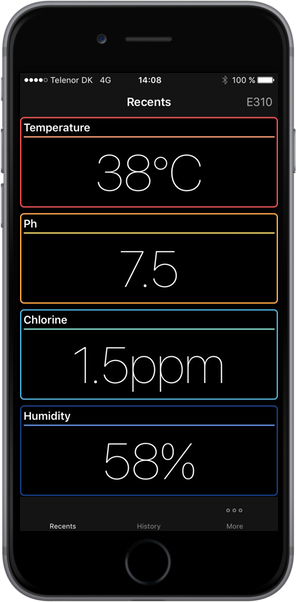
\includegraphics[width=0.4\linewidth]{figs/implementering/ios_imp_statview}
	\caption{iOS StatView}
	\label{fig:ios_imp_statview}
\end{figure}

\subsubsection{HistoryViewBridge.cs}
HistoryViewBridge implementerer IHistoryView-interfacet. HistoryViewBridge nedarver, ligesom StatViewBridge, fra UITableViewController. I listing~\ref{code:ios_impl_historydisplay} ses implementeringen af interface-metoden DisplayHistoricData. I denne metode gemmes den modtagne sensor data, så den kan bruges som data source til UITableViewController-listen.

\begin{lstlisting}[caption={DisplayHistoricData(...)},label={code:ios_impl_historydisplay}]
public void DisplayHistoricData(List<Tuple<SensorTypes, List<double>>> historicData)
{
	_historicData = historicData;
	_historicData.Sort ();
	TableView.ReloadData ();
}
\end{lstlisting}

Klassen overrider en række af UITableViewController-klassens metoder, der indlæser data i view'et. De overrides der bestemmer indholdet af listens elementer, fremgår af listing~\ref{code:ios_impl_historytableor}. I GetCell-metoden opsættes en HistoryViewCell (HistoryViewCell.xib), til at vise den data der er modtaget fra presenter-klassen.

\begin{lstlisting}[caption={Overrides af UITableViewController-metoder i HistoryViewBridge},label={code:ios_impl_historytableor}]
public override nint RowsInSection (UITableView tableView, nint section)
{
	return _historicData.Count;
}

public override UITableViewCell GetCell (UITableView tableView, Foundation.NSIndexPath indexPath)
{
	var cell = tableView.DequeueReusableCell (_reuseIdentifier) as HistoryViewCell;
	var type = string.Format ($"{_historicData [indexPath.Row].Item1}");
	cell.TypeLabel.Text = type;
	cell.BorderImage.Image = UIImage.FromFile (type.ToLower () + ".png");
	var bounds = DrawGraph (cell.GraphView, _historicData [indexPath.Row].Item2, _historicData [indexPath.Row].Item1);
	cell.MinLabel.Text = string.Format($"{bounds.Item1}");
	cell.MaxLabel.Text = string.Format($"{bounds.Item2}");
	return cell;
}
\end{lstlisting}

Under opsætningen af cellen kaldes den private hjælpefunktion DrawGraph, som har til formål at tegne en graf i cellen. I listing~\ref{code:ios_impl_historydrawgraph} viser implementeringen af DrawGraph-metoden. I metoden bruges en UIBezierPath til at tegne den serie af streger, som grafen består af.

\begin{lstlisting}[caption={DrawGraph(...)},label={code:ios_impl_historydrawgraph}]
private Tuple<double, double> DrawGraph(UIView view, List<double> values, SensorTypes type)
{
	var bounds = GraphBounds (values, (type == SensorTypes.Chlorine || type == SensorTypes.Ph));
	var points = GraphPoints (values, bounds, view);
	var numberOfPoints = points.Count;

	if (numberOfPoints == 0)
		return bounds;

	var path = new UIBezierPath ();
	path.MoveTo (points[0]);

	for (var i = 1; i < numberOfPoints; i++)
		path.AddLineTo (points[i]);

	var layer = new CAShapeLayer ();
	ayer.Path = path.CGPath;
	layer.StrokeColor = UIColor.White.CGColor;
	layer.LineWidth = 2;
	layer.FillColor = UIColor.Clear.CGColor;

	view.Layer.Sublayers = null;
	view.Layer.AddSublayer (layer);

	return bounds;
}
\end{lstlisting}

DrawGraph-metoden beregner punkterne i grafen, ud fra det sæt af data der modtages fra presenteren, ved at kalde hjælpefunktionen GraphPoints, listing~\ref{code:ios_impl_historygraphpoints}. Algoritmen i GraphPoints er en modificeret udgave af den, der blev lavet til Windows-implementeringen af IHistoryView-interfacet.

\begin{lstlisting}[caption={GraphPoints(...)},label={code:ios_impl_historygraphpoints}]
private List<CGPoint> GraphPoints(List<double> values, Tuple<double, double> bounds, UIView view)
{
	var points = new List<CGPoint> ();
	var numberOfPoints = values.Count;

	// Bounds
	var lowerBound = bounds.Item1;
	var upperBound = bounds.Item2;

	// Canvas size
	var canvasWidth = view.Frame.Width;
	var canvasHeight = view.Frame.Height;

	// Holds last point drawn. Is used to draw tendency line
	var lastPointX = 0d;
	ar lastPointY = 0d;

	// Draw graph
	for (var i = 0; i < numberOfPoints; i++)
	{
		var pointHeight = ((upperBound - values[i])) / (upperBound - lowerBound) * canvasHeight;
		var pointWidth = (canvasWidth/(numberOfPoints - 1))*i;

		var point = new CGPoint ();
		point.X = (nfloat)pointWidth;
		point.Y = (nfloat)pointHeight;
		
		points.Add (point);

		//Remember info on point for drawing the tendency line
		lastPointY = pointHeight;
		lastPointX = pointWidth;
	}

	return points;
}
\end{lstlisting}

På figur~\ref{fig:ios_imp_historyview} ses det visuelle resultat, af HistoryViewBridge implementeringen, når data vises i listen.

\begin{figure}
	\centering
	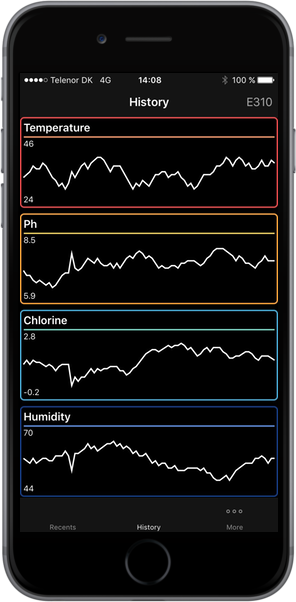
\includegraphics[width=0.4\linewidth]{figs/implementering/ios_imp_historyview}
	\caption{iOS HistoryView}
	\label{fig:ios_imp_historyview}
\end{figure}

\subsection{Implementering af iOS socket-klienten}
Da iOS-applikationen ikke kan drage nytte af det fulde .Net-framework, skulle en platform-specifik socket-klient implementeres. I stedet bruges biblioteket SocketLibrary, som er fundet med NuGet-package manager. Socket-klienten er en modificeret udgave af .Net-socket clienten, som beskrives i Connection afsnittet.

Socket-klienten implementerer IClient-interfacet, der er defineret i Smartpool.Connection.Model. iOS tillader en maksimal socket buffer-størrelse, på 1kb. Derfor implementeres StartClient-metoden (se listing~\ref{code:ios_impl_client}) i IClient-interfaet således, at den modtager data fra serveren af flere omgange. For at bufferen kan nå at modtage data mellem hver transmission, indsættes et mindre delay.

\begin{lstlisting}[caption={StartClient(...)},label={code:ios_impl_client}]
public string StartClient(string whatToSend)
{
	// Connect to a remote device.
	try
	{
		// Establish the remote endpoint for the socket.
		IPAddress ipAddress = IPAddress.Parse(_serverIp);
		IPEndPoint remoteEP = new IPEndPoint(ipAddress, 11000);

		// Create a TCP/IP  socket.
		var sender = new ConnectedSocket(remoteEP); 

		// Connect the socket to the remote endpoint. Catch any errors.
		try
		{
			// Send the data through the socket.
			sender.Send(whatToSend);

			// Receive the response from the remote device.
			var received = "";
			do {
				received += sender.Receive(1024);
				Thread.Sleep(20);
			}
			while (sender.AnythingToReceive);
			return received;
		}
		catch (Exception)
		{
			return JsonConvert.SerializeObject(new LoginResponseMsg("", false) { MessageInfo = "Error - Server did not respond\nMake sure server is started and Emil isn't nearby" }, _jsonSettings);
		}
	}
	catch (Exception)
	{
		return JsonConvert.SerializeObject(new LoginResponseMsg("", false) {MessageInfo = "Error - Server did not respond\nMake sure server is started and Emil isn't nearby"}, _jsonSettings);
	}
}
\end{lstlisting}